\documentclass{beamer}
\usetheme{CambridgeUS}
\usecolortheme{rose}
\usepackage[slovene]{babel}
\usepackage{graphicx}
\usepackage{subcaption}
\setbeamercolor{block title}{bg=red!20,fg=black}
\setbeamertemplate{caption}[numbered]

\title{Predstavitev pri predmetu - NRO}
\subtitle{1.DN}
\author{Gašper Kostelec}
\institute[] { 
Univerza v Ljubljani \\
Fakulteta za strojništvo \\
RRP, 3.letnik \\}
\date{\today}

\usepackage{tikz}
\titlegraphic { 
\begin{tikzpicture}[overlay,remember picture]
\node[right=0.2cm] at (current page.152){
    
\includegraphics[width=2cm]{UNI-logo-in-FS-color-SLO-curve (1).jpg}};
\end{tikzpicture}}


\begin{document}


\begin{frame}
    \titlepage
\end{frame}

\begin{frame}{Kazalo}
    \tableofcontents
\end{frame}

\AtBeginSection[ ]{
\begin{frame}{Kazalo}
    \tableofcontents[currentsection]
\end{frame}}



\section{Uvod in koda}

\begin{frame}{Uvod in kratek opis funkcij v kodi}
\begin{itemize}
    \item S pomočjo metode Monte Carlo smo v Matlab-u zapisali kodo(funkcije). Kodo smo nato nadgradili s sošolcem v Github-u in na koncu izdelali predstavitev v okolju Beamer.
\pause
    \item calc-pi() - v tej funkciji je zapisano začetno število točk, radij in kliče naslednjo funkcijo
\pause
    \item raziskuje-priblizke - ta funkcija pokliče vse potrebne funkcije in se izvede tolikokrat kot je zahtevano število-približkov. V tej funkciji je uporabljena tudi 'for' zanka.
\pause
    \item izrisi-graf() - pokliče svoji dve potrebni funkciji, in nariše graf za vsak približek posebej
\end{itemize}
\begin{figure}
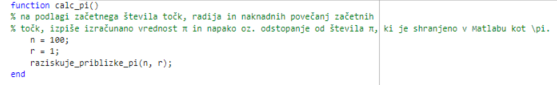
\includegraphics[scale=0.8]{začetek zapisa kode.png}
\caption{Začetna funkcija celotne datoteke}
\end{figure}
\end{frame}


\section{Grafi}

\begin{frame}{Prikaz grafov v odvisnosti od n}

\begin{columns}[T]
  \begin{column}{0.5\textwidth}
    \begin{figure}
      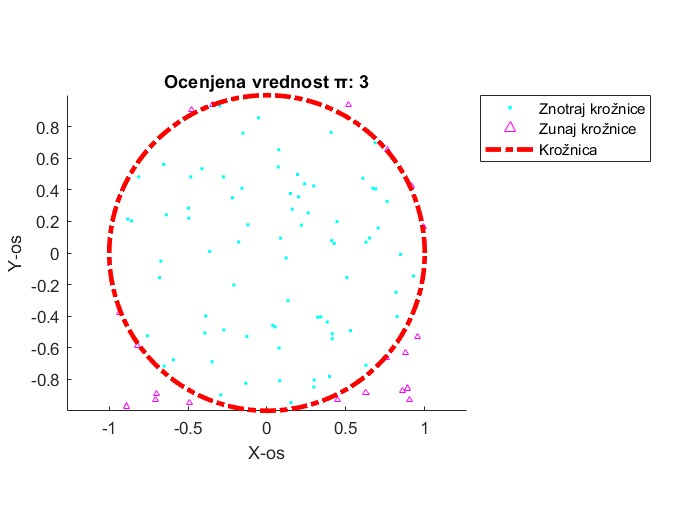
\includegraphics[width=.65\textwidth]{graf_1.jpg}
      \vspace*{-0.5cm}
      \caption{graf n=100}
    \end{figure}
  \end{column}
  \begin{column}{0.5\textwidth}
    \begin{figure}
      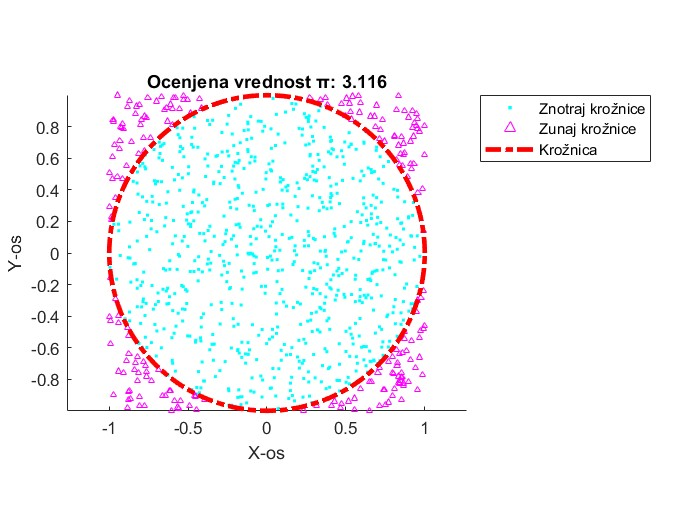
\includegraphics[width=.65\textwidth]{graf_2.jpg}
      \vspace*{-0.5cm}
      \caption{graf n*10}
    \end{figure}
  \end{column}
\end{columns}

\begin{columns}[T]
  \begin{column}{0.5\textwidth}
    \begin{figure}
      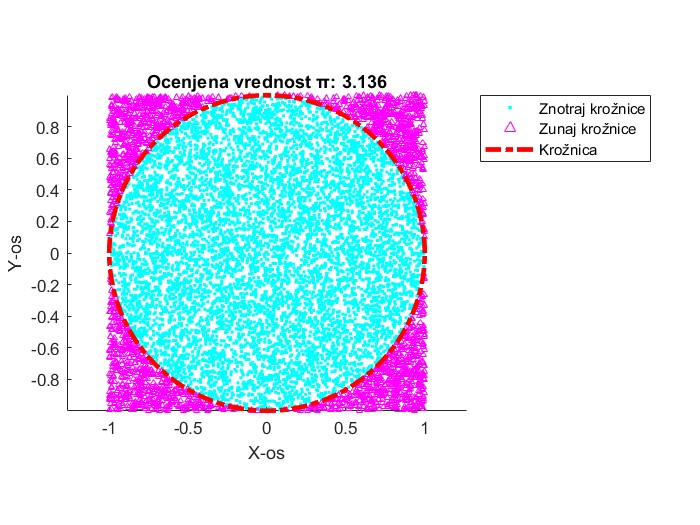
\includegraphics[width=.65\textwidth]{graf_3.jpg}
      \vspace*{-0.5cm}
      \caption{graf n*100}
    \end{figure}
  \end{column}
  \begin{column}{0.5\textwidth}
    \begin{figure}
      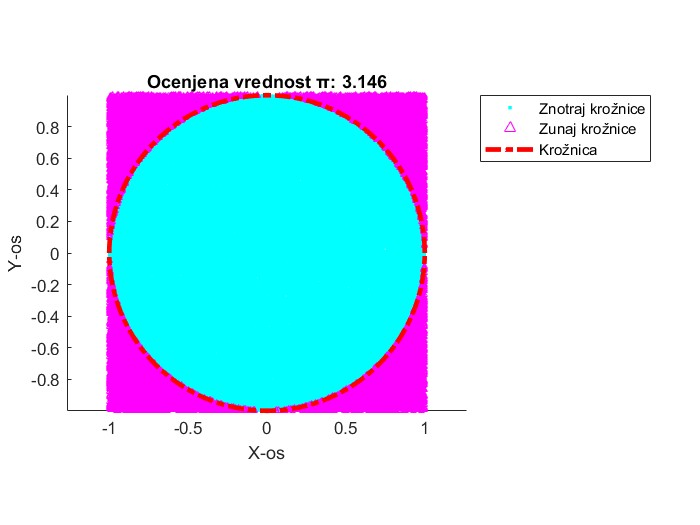
\includegraphics[width=.65\textwidth]{graf_4.jpg}
      \vspace*{-0.5cm}
      \caption{graf n*1000}
    \end{figure}
  \end{column}
\end{columns}
\end{frame}


\section{GitHub in Beamer}

\begin{frame}{Opis dela}
\begin{enumerate}
    \item k sodelavanju na projektu sem povabil asistenta in enega izmed sošolcev 
\pause
    \item sošolec je nato dopolnil nekaj podatkov glede izrisa grafa, katere sem po pregledu sprejel
\pause
    \item sledila je priprava predstavitve v okolju Beamer
\end{enumerate}

\begin{figure}
\centering
    \begin{subfigure}[b]{0.4\textwidth}
        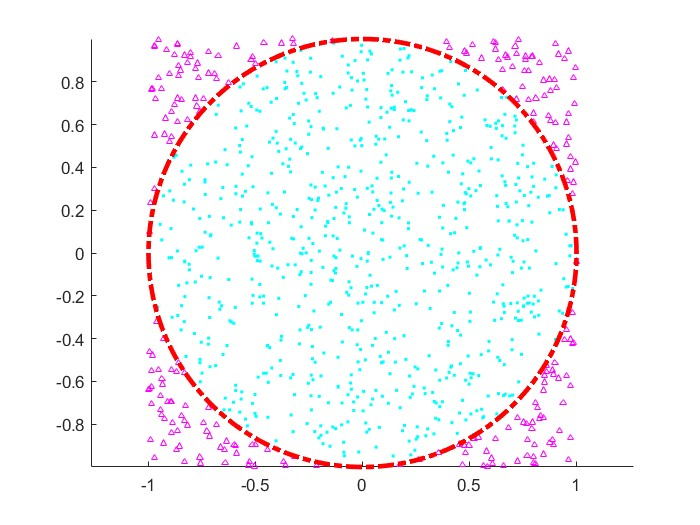
\includegraphics[width=0.6\textwidth]{graf_2 primerjava.jpg}
        \caption{Graf brez naslova, legende in poimenovanja osi}
    \end{subfigure}
    \begin{subfigure}[b]{0.4\textwidth}
        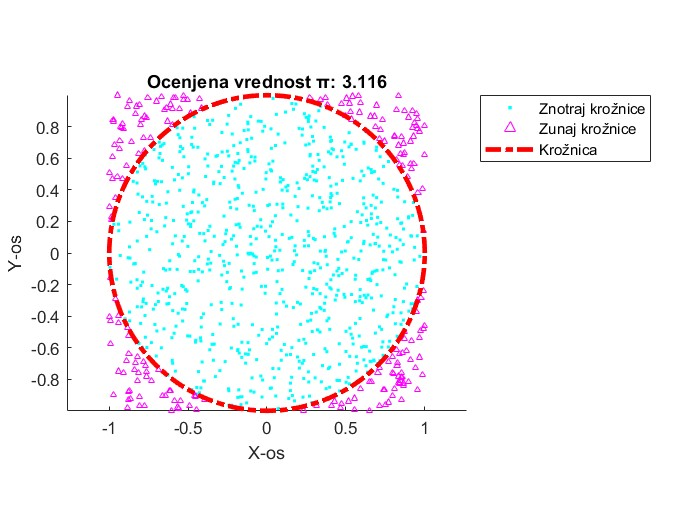
\includegraphics[width=0.78\textwidth]{graf_2.jpg}
        \caption{Ustrezno opremljen graf}
    \end{subfigure}
\caption{Primerjava grafov pred in po sodelovanju s sošolcem}
\end{figure}
\end{frame}


\section{Zaključek}

\begin{frame}{Tabela}
\begin{table}
\begin{tabular}{l | c | c | c | c }
približek & število točk & ocenjena vrednost & odstopanje \\
\hline \hline
1 & 100 & 3 & 0.14159 \\
\pause
2 & 1000 & 3.116 & 0.025593 \\
\pause
3 & 10000 & 3.136 & 0.0055927 \\
\pause
4 & 100000 & 3.146 & 0.0044473 
\end{tabular}
\caption{Prikaz rezultata enega izmed poiskusov iskanja vrednosti Pi}
\end{table}
S pomočjo zgornje tabele lahko opazimo, da z naraščajnem števila točk, dobimo tudi boljši približek vrednosti Pi.
\end{frame}



\end{document}
